\documentclass[a4paper,12pt]{article}
\usepackage{titlesec}
\usepackage{xcolor}
\usepackage{listings}
\usepackage{a4wide}                          
\usepackage{lipsum}
\usepackage{amsmath}                       
\usepackage{amsfonts}                      
\usepackage[pdftex]{graphicx}               
\usepackage{sidecap}                      
\usepackage{floatrow}        
\usepackage{subfig}            
\usepackage{fontawesome}
\usepackage[version=4]{mhchem}       
\usepackage{mathtools}
\usepackage{float}
\usepackage{flafter}
\usepackage[section]{placeins}
\usepackage{sidecap}                
\usepackage{floatrow} 
\usepackage{subfig}
\usepackage[framemethod=default]{mdframed}
\usepackage{capt-of}  
\usepackage{mhchem}
\usepackage[utf8]{inputenc}
\usepackage{graphicx}
\usepackage{fontenc}
\usepackage{mhchem}
\usepackage{siunitx}
\usepackage{tikz}
\usepackage{xcolor}
\usepackage{listings}
\usepackage{blindtext}
\usepackage[utf8]{inputenc}
\usepackage{placeins}
\usepackage[english]{babel}
\usepackage{geometry}
\usepackage{multicol}
\usepackage[T1]{fontenc}
\usepackage{tgbonum}
\usepackage{subfig}
\usepackage[LGRgreek]{mathastext}
\setlength{\columnsep}{8mm}
\FloatBarrier



 \geometry{
 a4paper,
 total={170mm,257mm},
 left=20mm,
 right=20mm,
 bottom=20mm,
 top=20mm,
 }


\floatsetup[table]{capposition=top}                                
\renewcommand{\tablename}{Table}                 


\title{{\sc Mandatory assignment 1 \\ {\large STK4900: Statistical Methods and Applications}}}

\author{Jamal Sharifi \\ }



\begin{document}
\linespread{1.5}
\renewcommand{\refname}{Referanser}
\renewcommand{\figurename}{Fig.} 

\onecolumn
\maketitle


%-----------------------------------------------------------------------------------------------------------------------------
\section*{Problem 1 }
In this exercise we are asked to study how air pollution at a measuring station at Alnabru in Oslo is related to explanatory variables traffic volume and meteorological conditions in the same place. The data set we are given consist of 500 observations collected by the Norwegian Public Roads Administration(Vegvesenet). The variables in the data set are

\begin{table}[H]
\caption*{} 
\centering
\begin{tabular}{l l} 
 log.no2 & The logarithm of the concentration of NO2  \\ [0.5ex] 
log.cars   & The logarithm of the number of cars per hour \\  
temp & Temperature 2 meters above the ground (degrees C) \\ 
wind.speed & Wind speed (meters/second) \\ 
hour.of.day & Hour of the day the measurements were collected (1-24) \\ [1ex] 
\end{tabular}
\end{table}

\subsection*{A. }
Main features of the variables log.no2 and log.cars are summarized in the table 1.

\begin{table}[H]
\caption{Summaries of the variables log.no2 and log.cars.} 
\centering
\begin{tabular}{c c c c c c c} 
\hline\hline 
 & Min & 1st Qu. & Median &  Mean  & 3rd Qu. &  Max.        \\ [0.5ex] 
\hline 
log.no2 & 1.224  & 3.214  & 3.848 &  3.698  & 4.217 &  6.395 \\  
log.cars & 4.127 &  6.176 &  7.425 &  6.973 &  7.793 & 8.349 \\ [1ex] 
\hline\hline
\end{tabular}
\end{table}

These numerical values can also be visualized for each variable by boxplots, as shown in the figures below. Here the thick line represents the median, Q1 and Q3 are the lines below and above the box containing the median. There is also a minimum and maximum line. Any values falling outside min and max represent 0.35 \% of the values.

\begin{figure}[H]
\subfloat[Boxplot for the variable log.no2.]{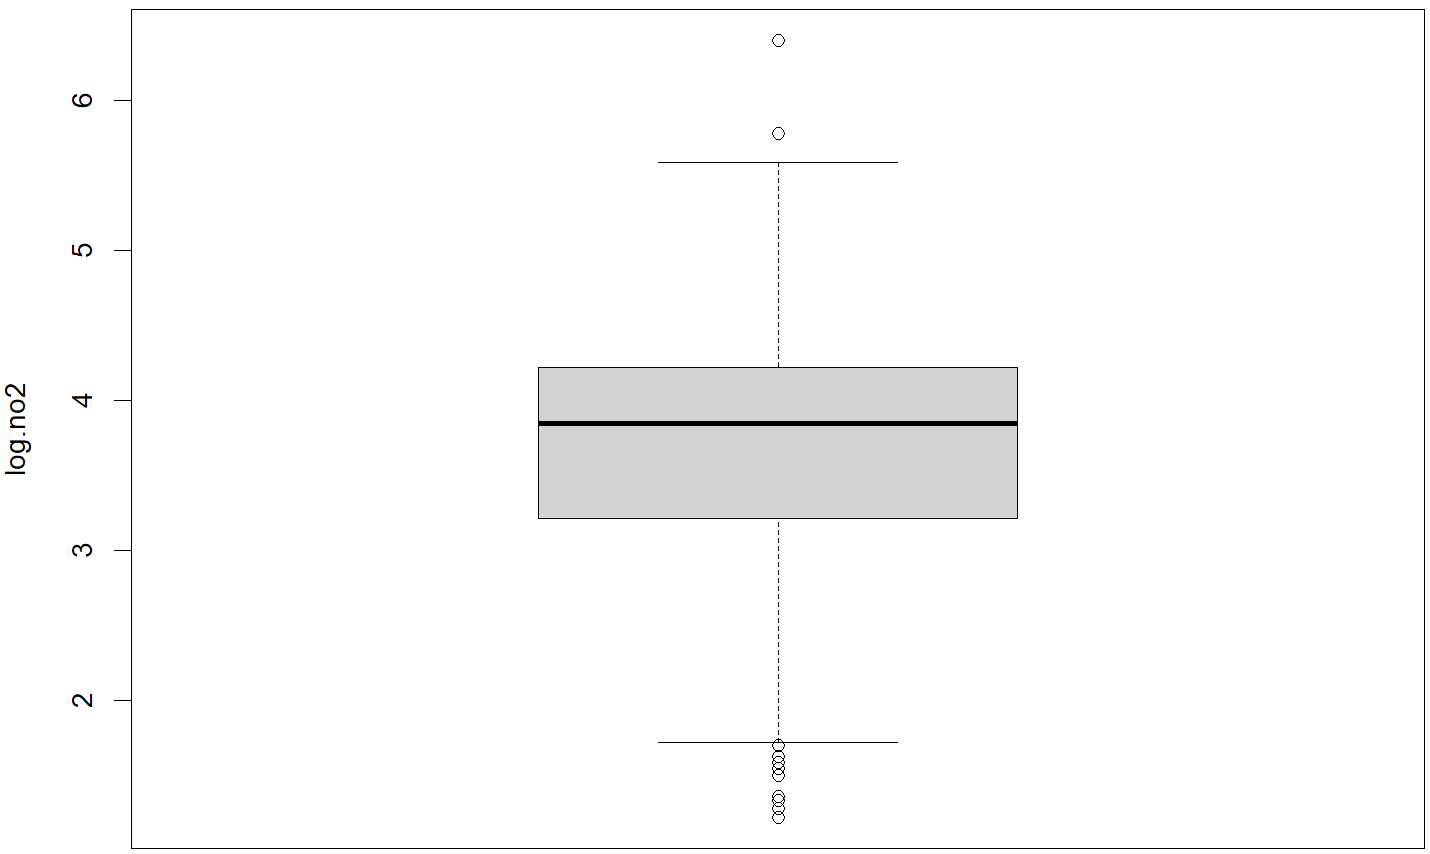
\includegraphics[width=3.2in, height=2in]{boxplot(A1).png}}
\subfloat[Boxplot for the variable log.cars.]{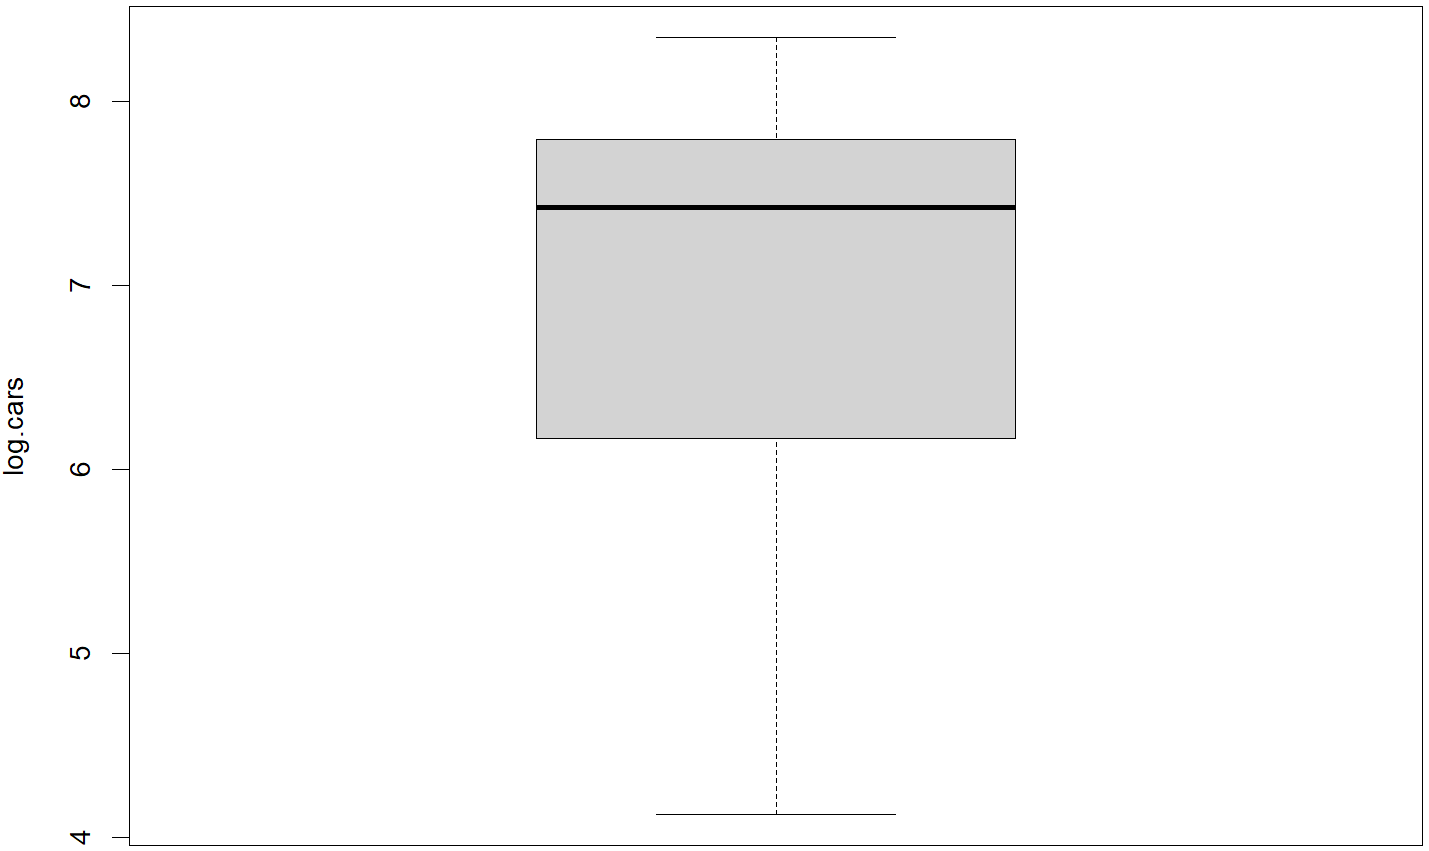
\includegraphics[width=3.2in, height=2in]{boxplot(A2).png}}
\caption{Boxplots for the two variables.}
\end{figure}



Figure below shows scatterplot, with log.no2 on y-axis and log.cars on the x-axis.  The figure shows increase in log($NO_2$) with increasing number of cars. Comparing the scatterplot we can see that the concentration of points are distributed accordingly both to the numerical values listed in table 1 and the boxplots. Further, there seems to be a clear correlation between the two variables.

\begin{figure}[H]
\centerline{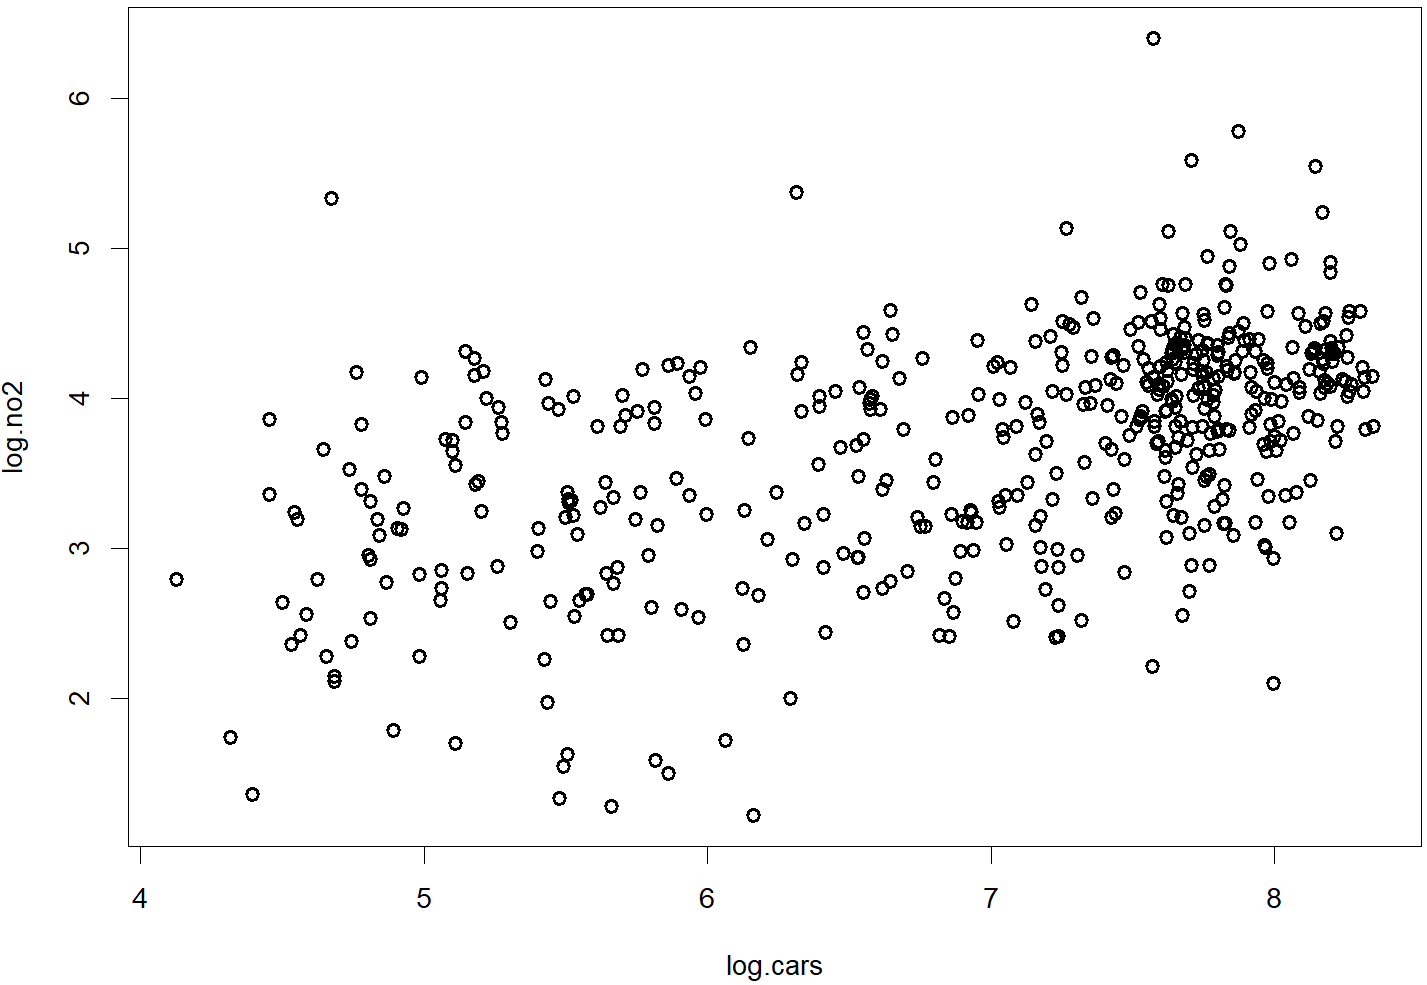
\includegraphics[width=4.5in, height=2.5in]{Scatterplot(A).png}}
\caption{Scatterplot of log.no2 vs log.cars.}
\label{fig}
\end{figure}





\subsection*{B. }
The simple linear model is described by

\begin{equation}
y_i=\beta_0+\beta_1x_i+\epsilon_i, \quad i=1,...,n
\end{equation}

Where $y_i$ are the outcomes and $x_i$ are the variables. For this particular set up the concentration of $log(NO_2)$ responds to the predictors which are number of cars per hour. The slope of this line is $\beta_1$ and the intersection is $\beta_0$, finally $\epsilon_i$ are the residuals.\\

Like the solution in A., we find the numerical values for this model and then we plot it. 

\begin{table}[H]
\caption{Coefficients of the simple linear model.} 
\centering 
\begin{tabular}{c c c c c c } 
\hline\hline 
 & Estimate Std. & Error & t value &  Pr(>|t|)          \\ [0.5ex] 
\hline 
Intercept & 1.23310  & 0.18755  & 6.575 &  1.23e-10   \\ 
log.cars & 0.35353 &  0.02657 &  13.303 &  < 2e-16   \\ [1ex] 
\hline 
\multicolumn{6}{c }{Residual standard error: 0.6454 on 498 degrees of freedom }\\
\multicolumn{6}{c }{Multiple R-squared:  0.2622,	Adjusted R-squared:  0.2607 }\\
\multicolumn{6}{c }{F-statistic:   177 on 1 and 498 DF,  p-value: < 2.2e-16 }\\
\hline\hline
\end{tabular}
\end{table}


Using the numerical values for the coefficients listed in table 2 together with eq. (1), the simple linear model is then

\begin{equation}
log.NO_2=1.23310+0.35353(log.cars)+\epsilon, \quad i=1,...,n
\end{equation}

$R^2$ is the square of the Pearson correlation coefficient, it a measure of goodness of a fit. It can have values ranging from 0 to 1. With 0 the model cannot explain any response data, and with 1 it explains all the response data\\

Looking at table 2, we can see that the p - value is close to 0. This suggest that there is a linear relationship between the variables. However the residual standard error is very large and $R^2$ is relatively small, and therefore the model might not be a good fit. There is also the possibility that $log.NO_2$ is not describes by $log.cars$ alone, by including other predictors we might get a better fit.

\begin{figure}[H]
\centerline{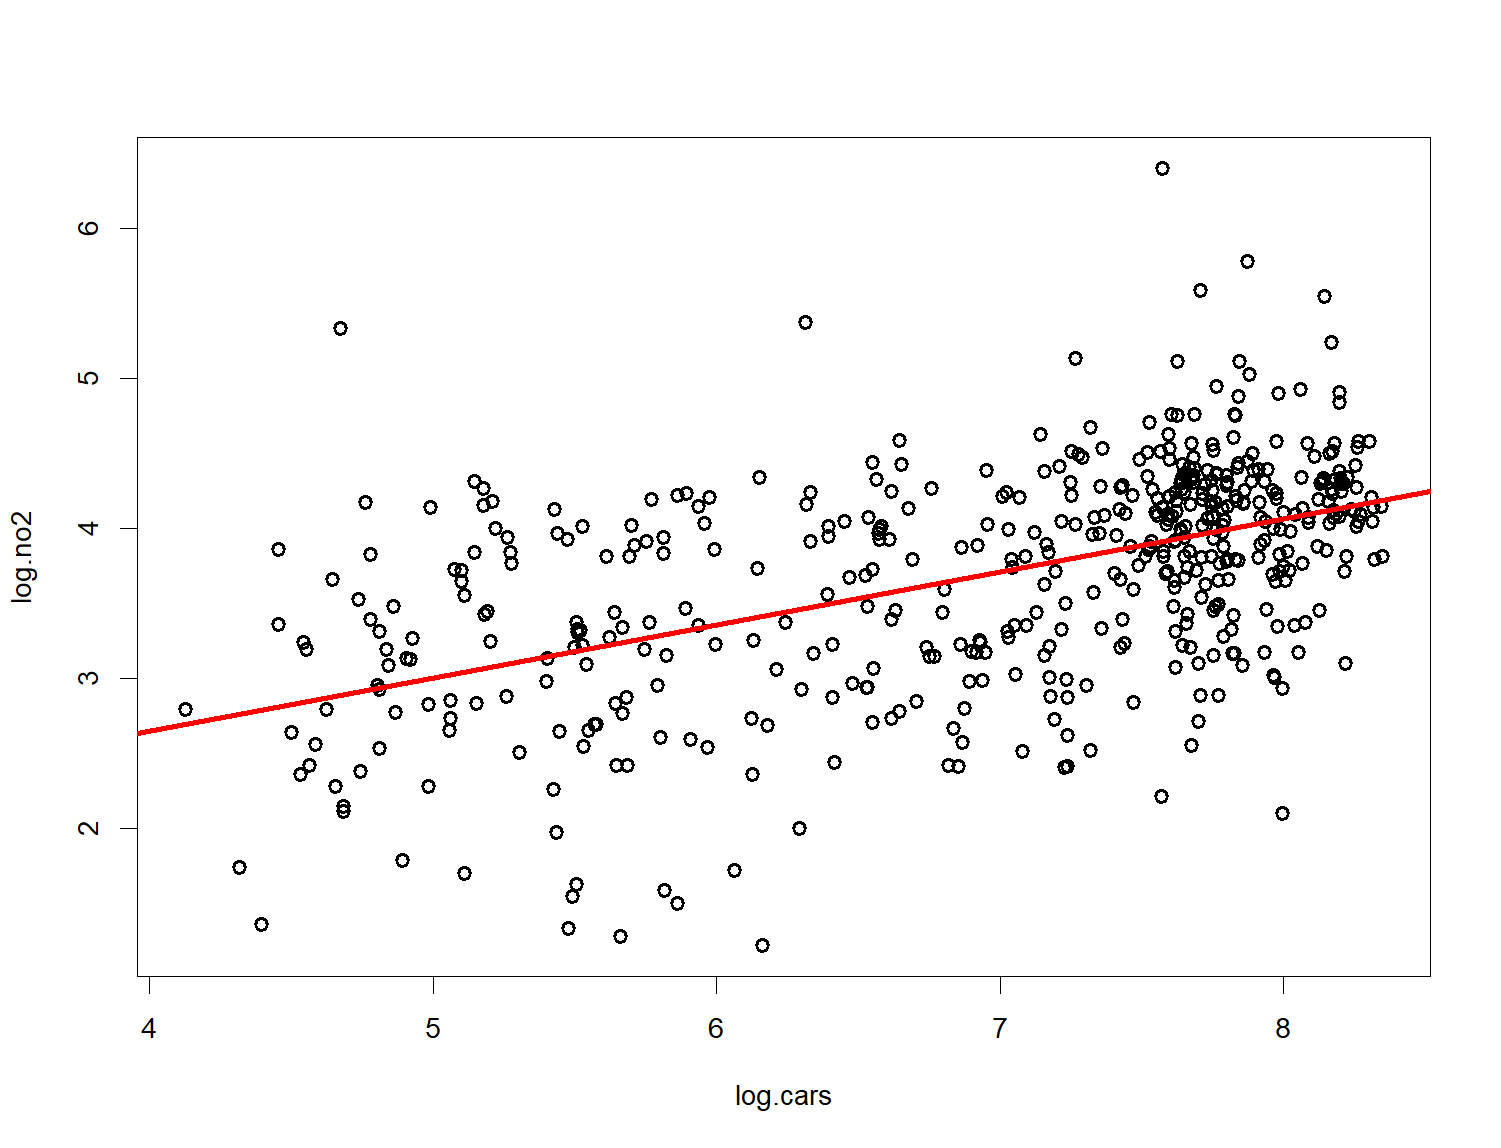
\includegraphics[width=4.5in, height=2.5in]{Fit_scatterplot(B).png}}
\caption{The simple linear model together with the scatterpoints.  }
\label{fig}
\end{figure}

\subsection*{C. }
A linear model for one predictor has the form of eq. (1). To see if our assumed linear model holds, we check linearity by looking at a CPR plot. Here we will have  Residuals + $\beta_i log.NO_2$ on y-axis and $log.NO_2$ on the x-axis.\\




\begin{figure}[H]
\centerline{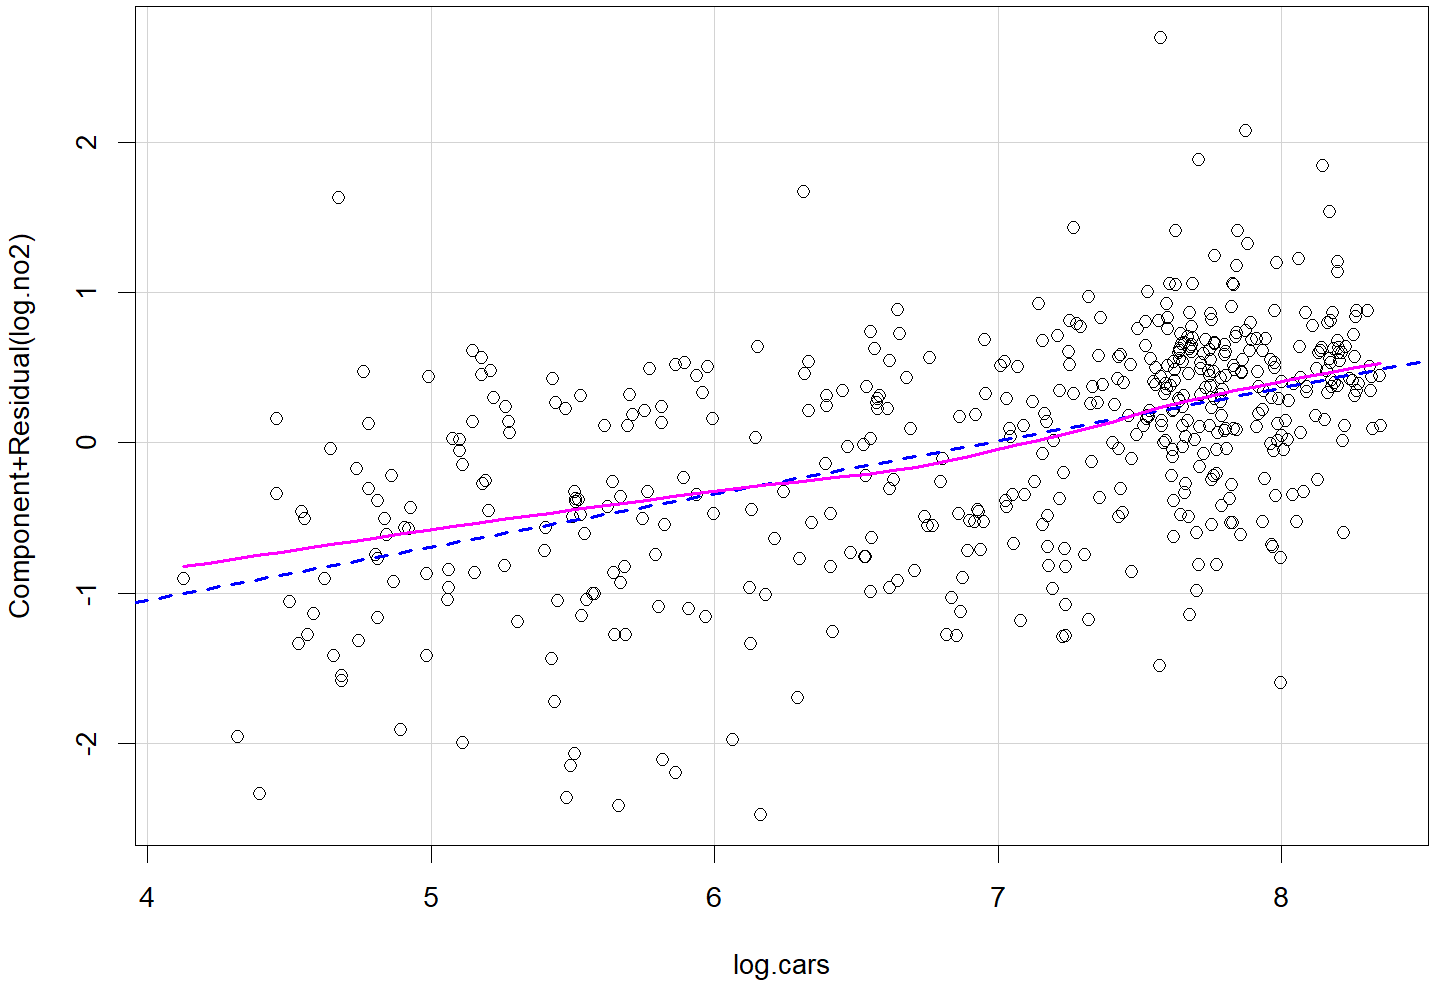
\includegraphics[width=4.5in, height=3in]{crPlot(C).png}}
\caption{Component + residuals vs log.cars. The straight line is our model, and the pink curve are the errors.}
\label{fig}
\end{figure}

From figure 3, we can see that the data points are more spread out for smaller values of log.cars. This better illustrated with a CPR plot in the figure above. Here we see the residuals deviates some places from the linear model. However, this deviation is not significant enough to conclude that it is a completely non-linear model.\\

Our model should also have normally distributed residuals, that is to say that all the residuals have the same constant variance. So we check for homoscedasticity, this can be done by plotting $\sqrt{SR}$ vs fitted values. If this is true, then we should be able to fit a straight line with no slope through the data points. 

\begin{figure}[H]
\centerline{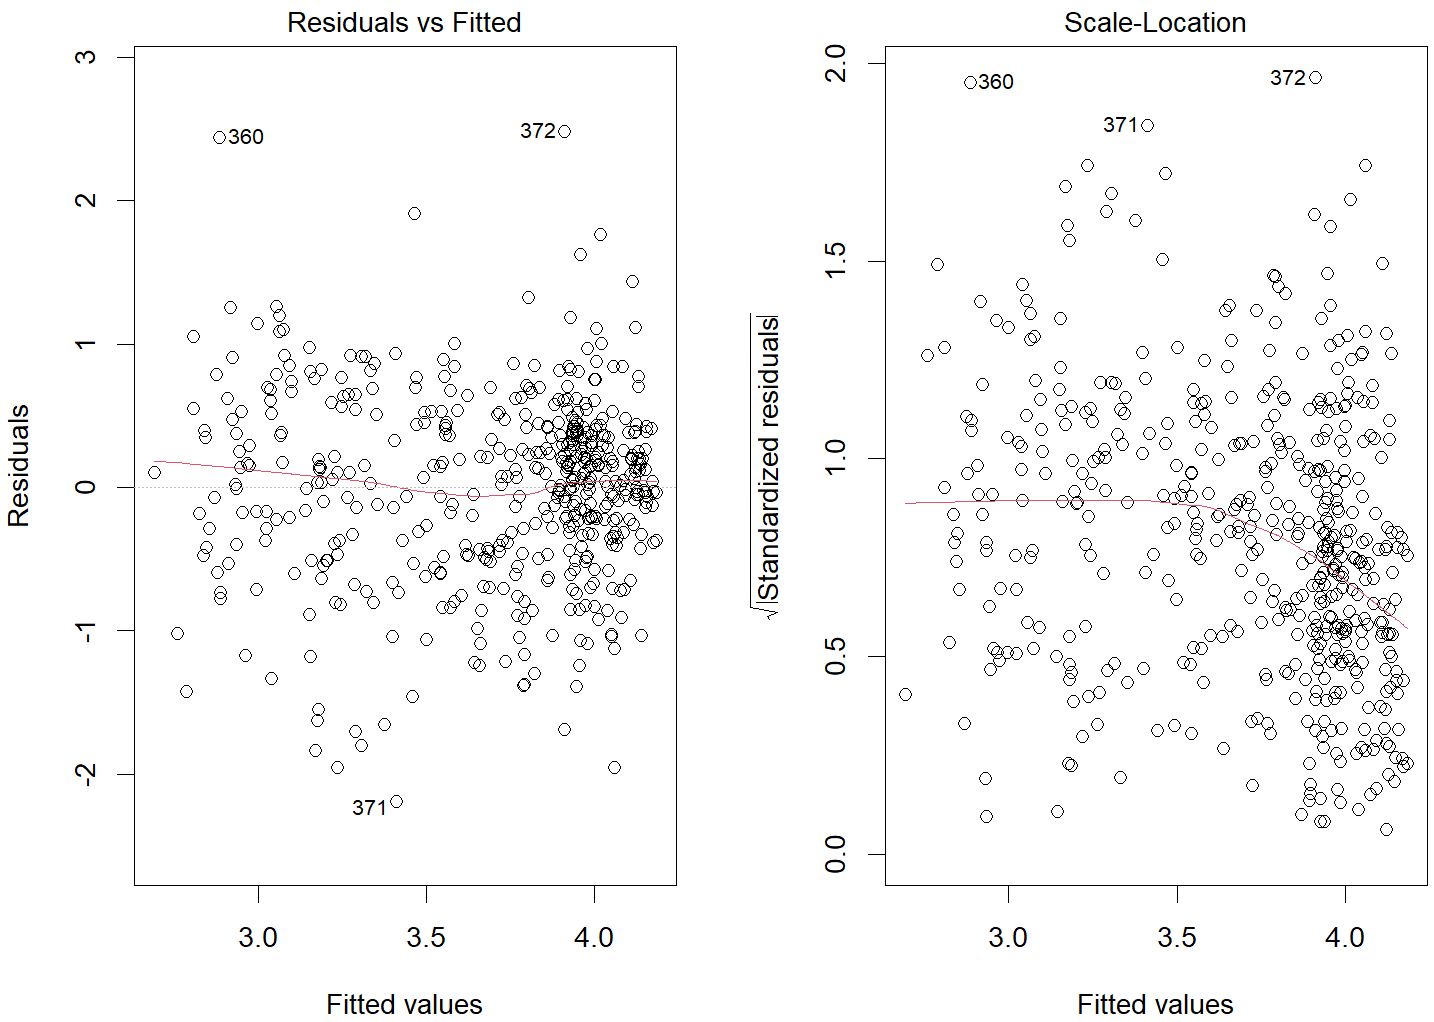
\includegraphics[width=4.5in, height=3in]{residualsStandard(C).png}}
\caption{Residual plots with fitted lines (red curve).}
\label{fig}
\end{figure}

The figure above shows that constant variance is presence until around 3.6 on the x-axis, after this the square root of the standardized residuals decreases. As discussed earlier this is due to data-points being more spread out for lower values.\\

Finally, we look for normality. This can be done by plotting a histogram together with a boxplot of the residuals, as shown in the figures blow. 

\begin{figure}[H]
\centerline{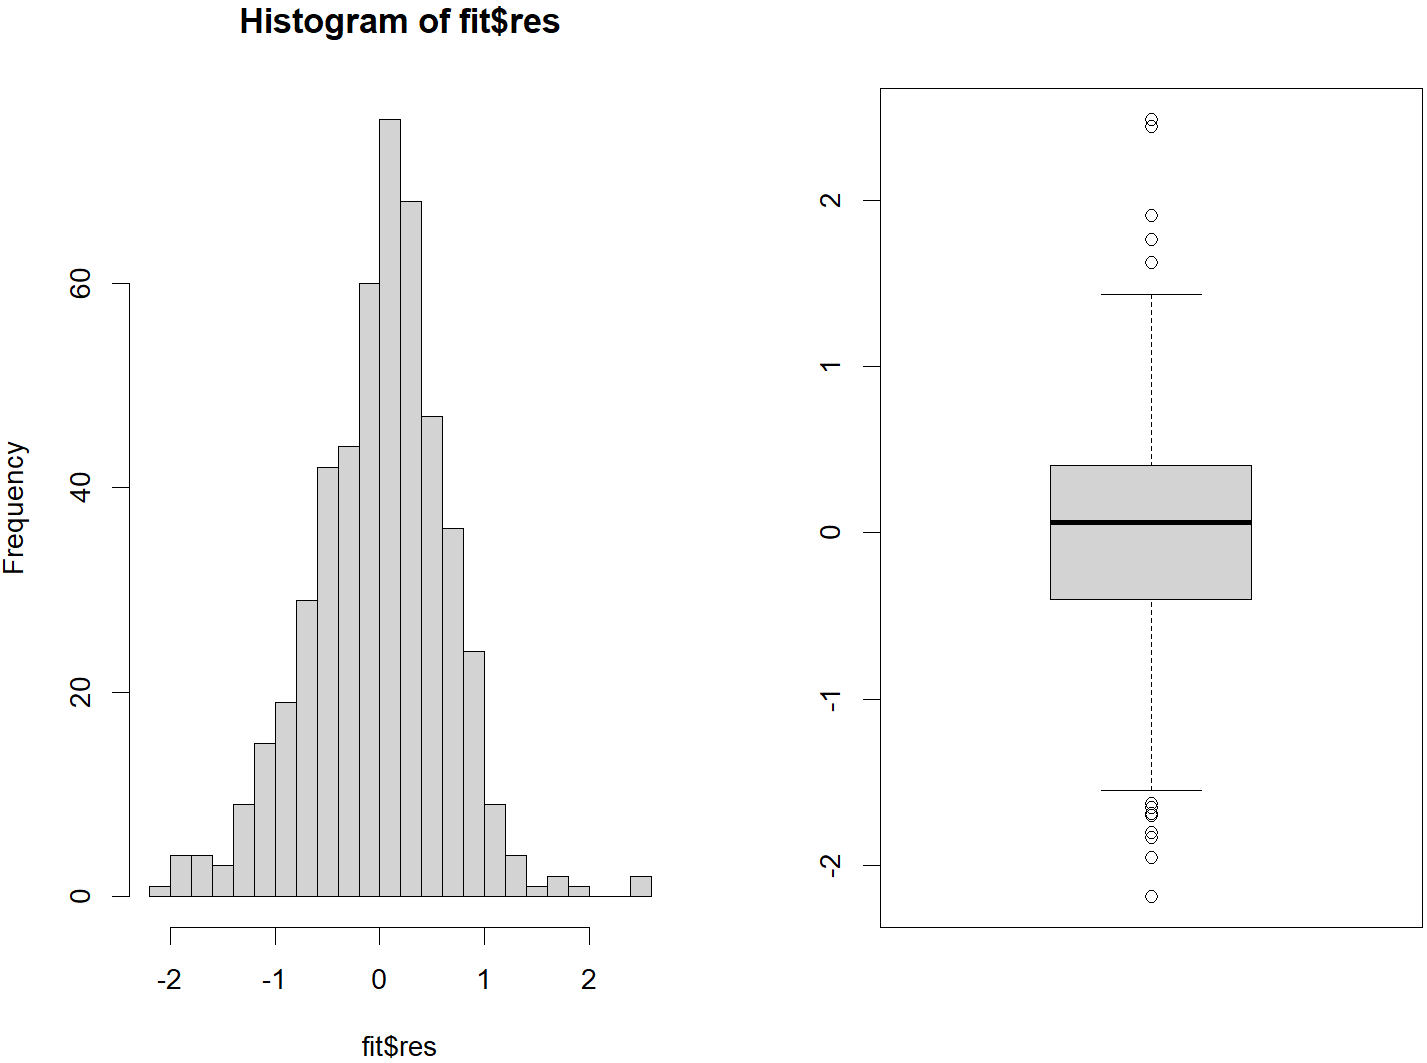
\includegraphics[width=4.5in, height=3in]{HistogramBoxplot(C).png}}
\caption{Histogram and boxplot of the residuals.}
\label{fig}
\end{figure}

In figure 6, we can see that the histogram is not symmetric, especially on the right side of the expected value. And the boxplot shows that the median is not at center in between 1st and 3rd quantile. Also here, the values that are not evenly spread from max and min points. Further, the expected value is not 0 in the histogram neither is the median. The shape of the histogram suggest that the residuals are normal distributed to some degree, although not completely normal distributed.

\begin{figure}[H]
\centerline{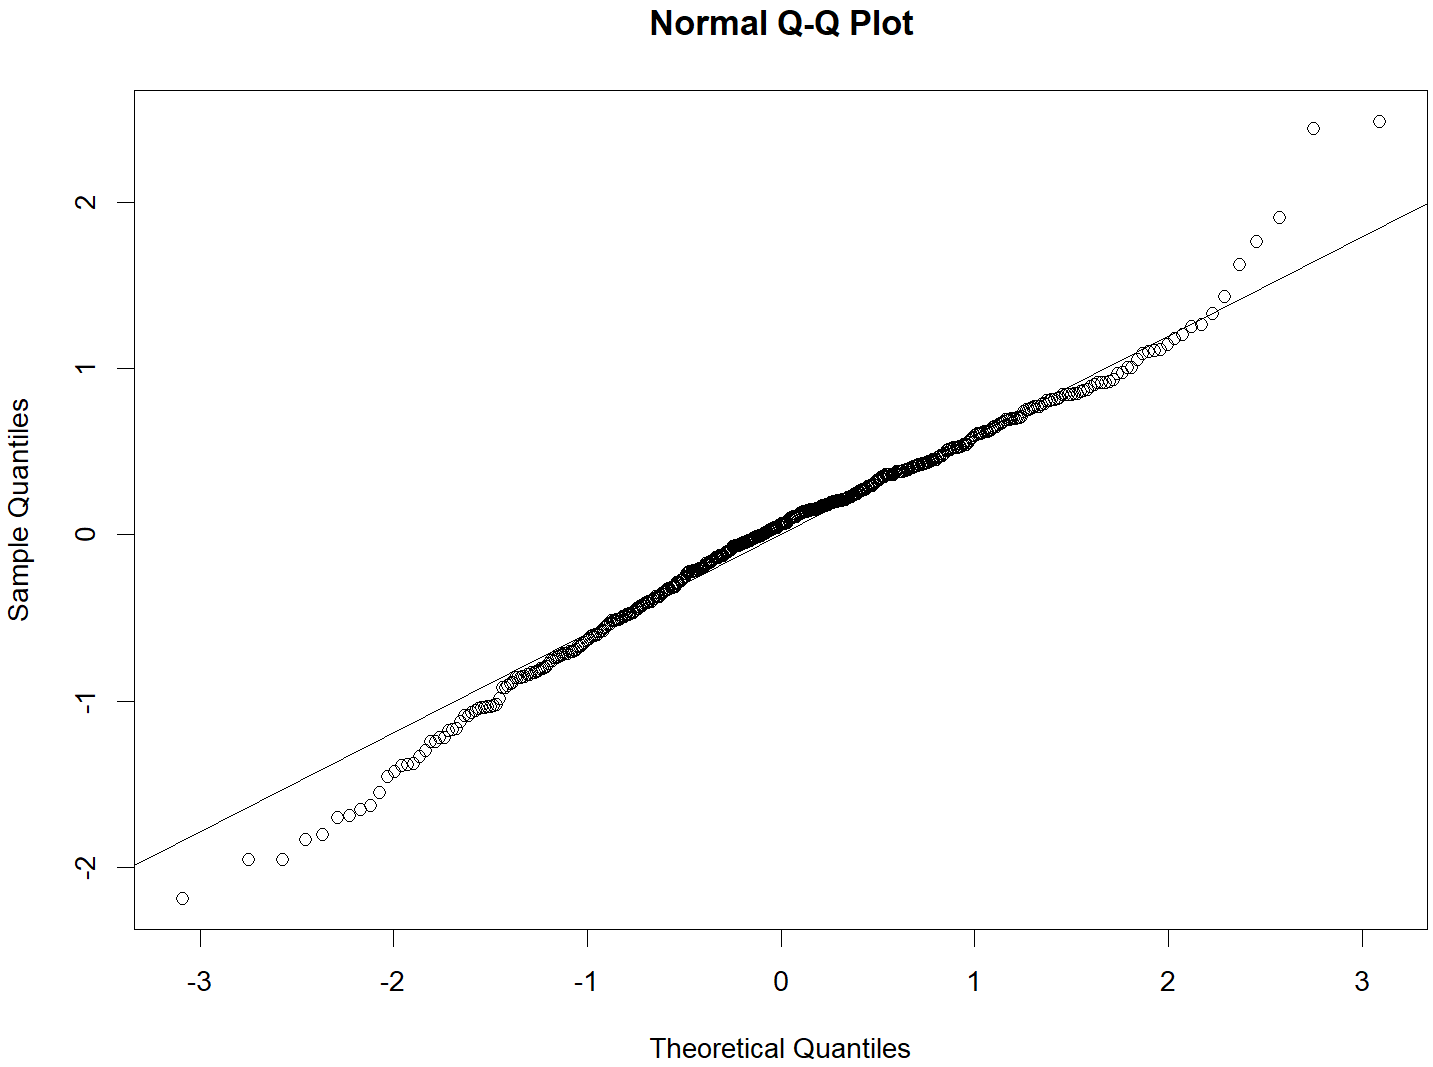
\includegraphics[width=4.5in, height=3in]{Q-Qplot.png}}
\caption{Q-q plot of the residuals.}
\label{fig}
\end{figure}

Upon further investigation of normality we look at the qq plot of residuals. Here, we should get a straight line through the points. But this not the case for the extreme values as it was also shown in the histogram. The arguments made for the linear model here suggests that there might be a better model that describes log.no2, that is to say log.no2 is depended on more than one predictor.


\subsection*{D. }
The best model can be found trough trial and error. Here we try different log transformation combination of the predictors and look at the adjusted $R^2$, and then choose the one combination that gives highest adjusted $R^2$. The different combinations are listed in the table below. The only variable that has not been log transformed is the temperature. This is because temperature contains some negative values, and the log of that does not exist. 

\begin{table}[H]
\caption{Fit models and their corresponding $R^2$ and adjusted $R^2$ coefficients.} 
\centering 
\begin{tabular}{c c c } 
\hline\hline 
 Model & $R^2$ & Adjusted $R^2$          \\ [0.5ex] 
\hline 
log.cars+temp+wind.speed + log(hour.of.day)        &0.4625   &0.4582    \\
log.cars+temp+wind.speed + hour.of.day               &0.4658   &0.4615   \\
log.cars+temp+log(wind.speed) + log(hour.of.day) &0.4807   &0.4766   \\
log.cars+temp+log(wind.speed) + hour.of.day        &0.4833   &0.4791  \\ [1ex] 
\hline\hline
\end{tabular}
\end{table}

From table 3, we can see that the last model gives best $R^2$ and adjusted $R^2$. This is the best linear model to describe log.no2 and its coefficients are listed in the table below. The best fit linear model therefore is


\begin{equation} 
\begin{split}
log.NO_2  = &\beta_0+\beta_1 log.cars+\beta_2 temp+\beta_3 log(wind.speed)+\beta_4 hour.of.day +\epsilon \\
  = & 1.070868+0.457188 \cdot log.cars - 0.026724 \cdot temp - \\ 
& 0.419388 \cdot log(wind.speed) - 0.012297 \cdot hour.of.day +\epsilon\\
\end{split}
\end{equation}

\begin{table}[H]
\caption{Coefficients of the simple linear model with 4 predictors.} 
\centering 
\begin{tabular}{c c c c c } 
\hline\hline 
 & Estimate & Std. Error & t value &  Pr(>|t|)          \\ [0.5ex] 
\hline 
(Intercept)      &1.070868   &0.170984   &6.263 &8.21e-10 \\
log.cars         &0.457188   &0.027931  &16.369  &< 2e-16 \\
temp            &-0.026724   &0.003837  &-6.964 &1.06e-11\\
log(wind.speed) &-0.419388   &0.036362 &-11.534  &< 2e-16 \\
hour.of.day     &-0.012297   &0.004374  &-2.811  &0.00513 \\ [1ex] 

\hline 
\multicolumn{5}{c }{Residual standard error: 0.5417 on 495 degrees of freedom }\\
\multicolumn{5}{c }{Multiple R-squared:  0.4833,	Adjusted R-squared:  0.4791 }\\
\multicolumn{5}{c }{F-statistic: 115.7 on 4 and 495 DF,  p-value: < 2.2e-16 }\\
\hline\hline
\end{tabular}
\end{table}



\subsection*{E. }
The CPR plot below shows that there seems to be good linearity between the residuals and the predictors. As with the model where only log.cars where include, here to we see that at the edges the residuals deviates so that it becomes non linear. However, overall the fitted lines looks to be close to the residuals for all the predictors. Finally looking at multiple $R^2 $ for the multi linear model we have 0.4833 which is a lot better than what we got when we used only one predictor. For this reasons, the models assumptions seems reasonably enough to conclude that it is indeed linear.

\begin{figure}[H]
\centerline{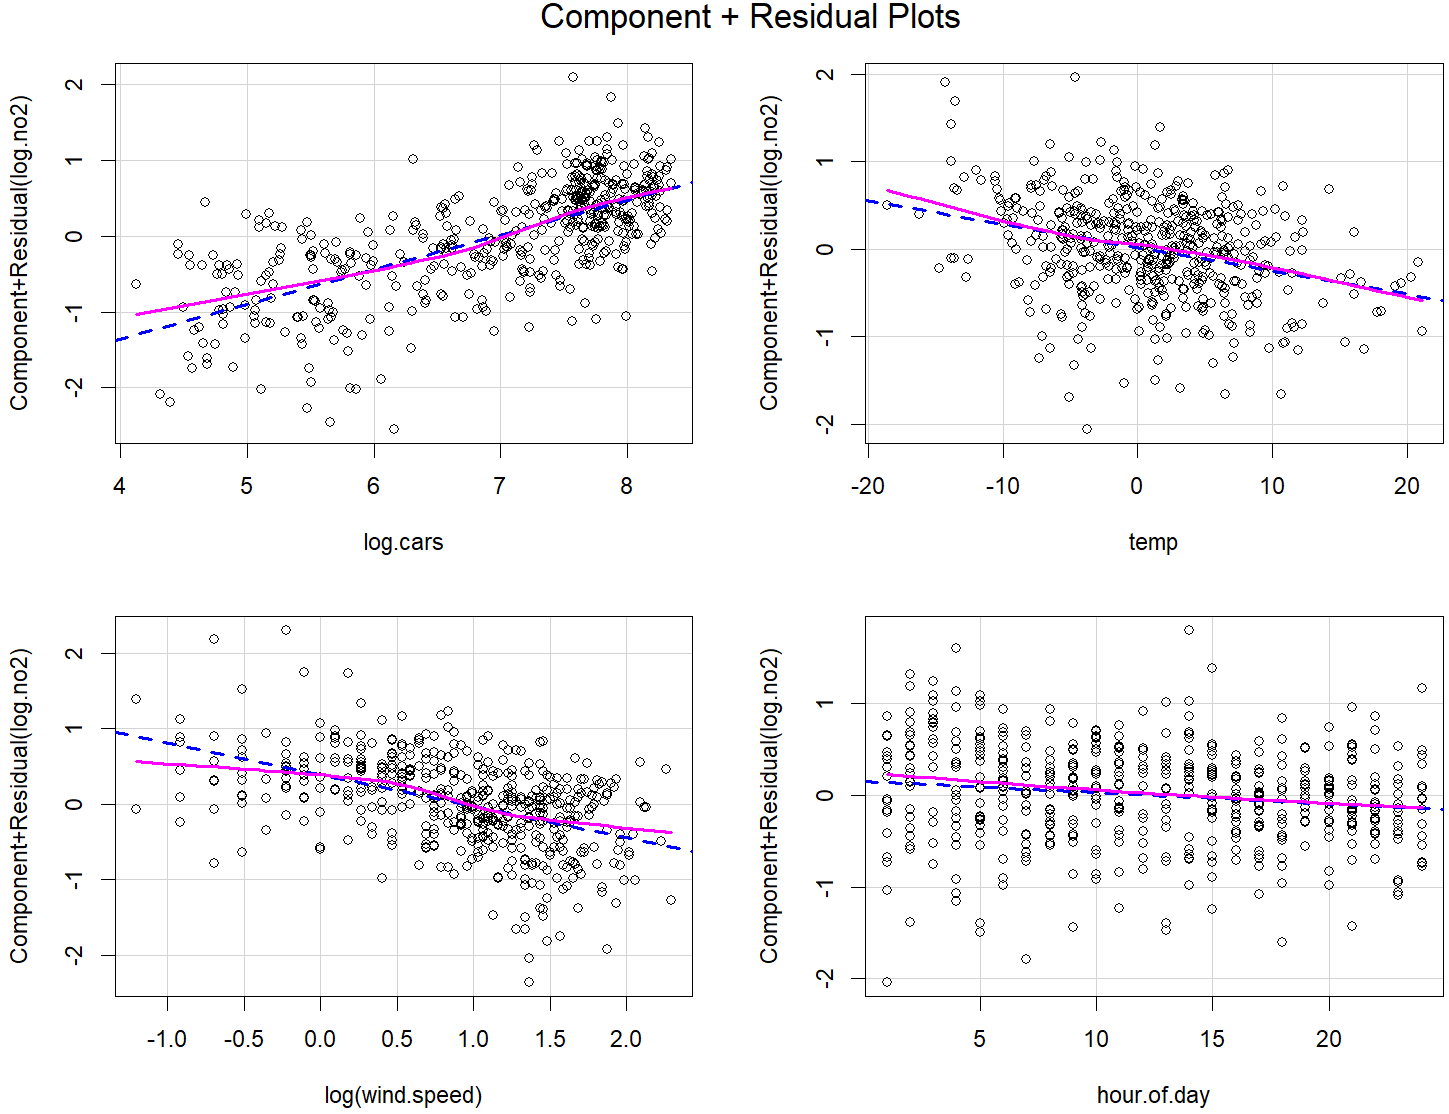
\includegraphics[width=5in, height=3in]{CPR_plot(D).png}}
\caption{CPR plot for the different variables.}
\label{fig}
\end{figure}

From table 4, lowest possible concentration of log($NO_2$) is 1.07 $\mu gm^-3 $. This is the lowest possible concentration of log($NO_2$) that can be in the air at any time, temperature and at any wind speed.  We can also see that all the coefficients are negative except for log.cars. This means increasing temperature, wind speed and the time has negative effect on air pollution. On average for each increase by 1 in log(cars), concentration will increase by 0.46 when the rest of the variables are held constant. For 1 increase in the temperature, concentration will decrease by 0.03 $\mu gm^-3 $. For 1 increase in log(wind speed) and 1 increase in hours we get rid of 0.42 and 0.01 $\mu gm^-3 $ log($NO_2$) respectively. 


\section*{Problem 2}
In this excersise we study the measurments of blood pressure of random samples of 12 men in three age groups. 

\begin{table}[H]
\caption*{} 
\centering
\begin{tabular}{|c | c | c|} 
\hline\hline
 30 - 45 years  & 46 - 59 years & 60 –75 years \\ [0.5ex] 
\hline
128, 104, 132, 112   & 120, 136, 174, 166 & 214, 146, 138, 148 \\  
\hline
136, 124, 112, 118 & 138, 124, 160, 157 & 156, 110, 188, 158 \\
\hline 
116, 108, 160, 116 & 108, 110, 154, 122 & 182, 148, 138, 136 \\ [1ex] 
\hline\hline
\end{tabular}
\end{table}

\subsection*{A. }

Looking at table 5, we see that clearly all the different data types are increasing with increasing age groups. Increase in the min is not as big as the increase in  max. Even in a small sample like this, the variation is not surprising. More importantly the average blood pressure is increasing by 20 from the age group 1 to age group 2, and by 11 from group 2 to group 3. So the increase between each group becomes smaller, however still significant. This is also true for 3rd. Qu., where 75 \% of the data lies. The differences between 1st. and 3rd. Qu. for each group varies also more with increasing age group. This suggests data for the blood pressure is more spread with increasing age. 

\begin{table}[H]
\caption{Summary of the different age groups.} 
\centering 
\begin{tabular}{c c c c c c c} 
\hline\hline 
 Age group & Min. & 1st Qu. &Median &  Mean & 3rd Qu. &Max.       \\ [0.5ex] 
\hline 
30 - 45 years (1)      &104   &112   &117 &122.2&129&160 \\
46 - 59 years (2)      &108   &121.5   &137 &139.1 &157.8&174 \\
60 - 75 years (3)      &110   &138   &148 &155.2&164&214 \\ [1ex] 
\hline\hline
\end{tabular}
\end{table}

We can now compare the numerical values summarized in table 5 with the boxplot under. Just like the numerical values listed in table 5, we see that the data is more spread out with increasing age group. For age group 1 and 3 we can see that the median is closer to 1st Qu. than it is for age group 2. That means there are more individuals with lower blood pressure than with high blood pressure. 



\begin{figure}[H]
\centerline{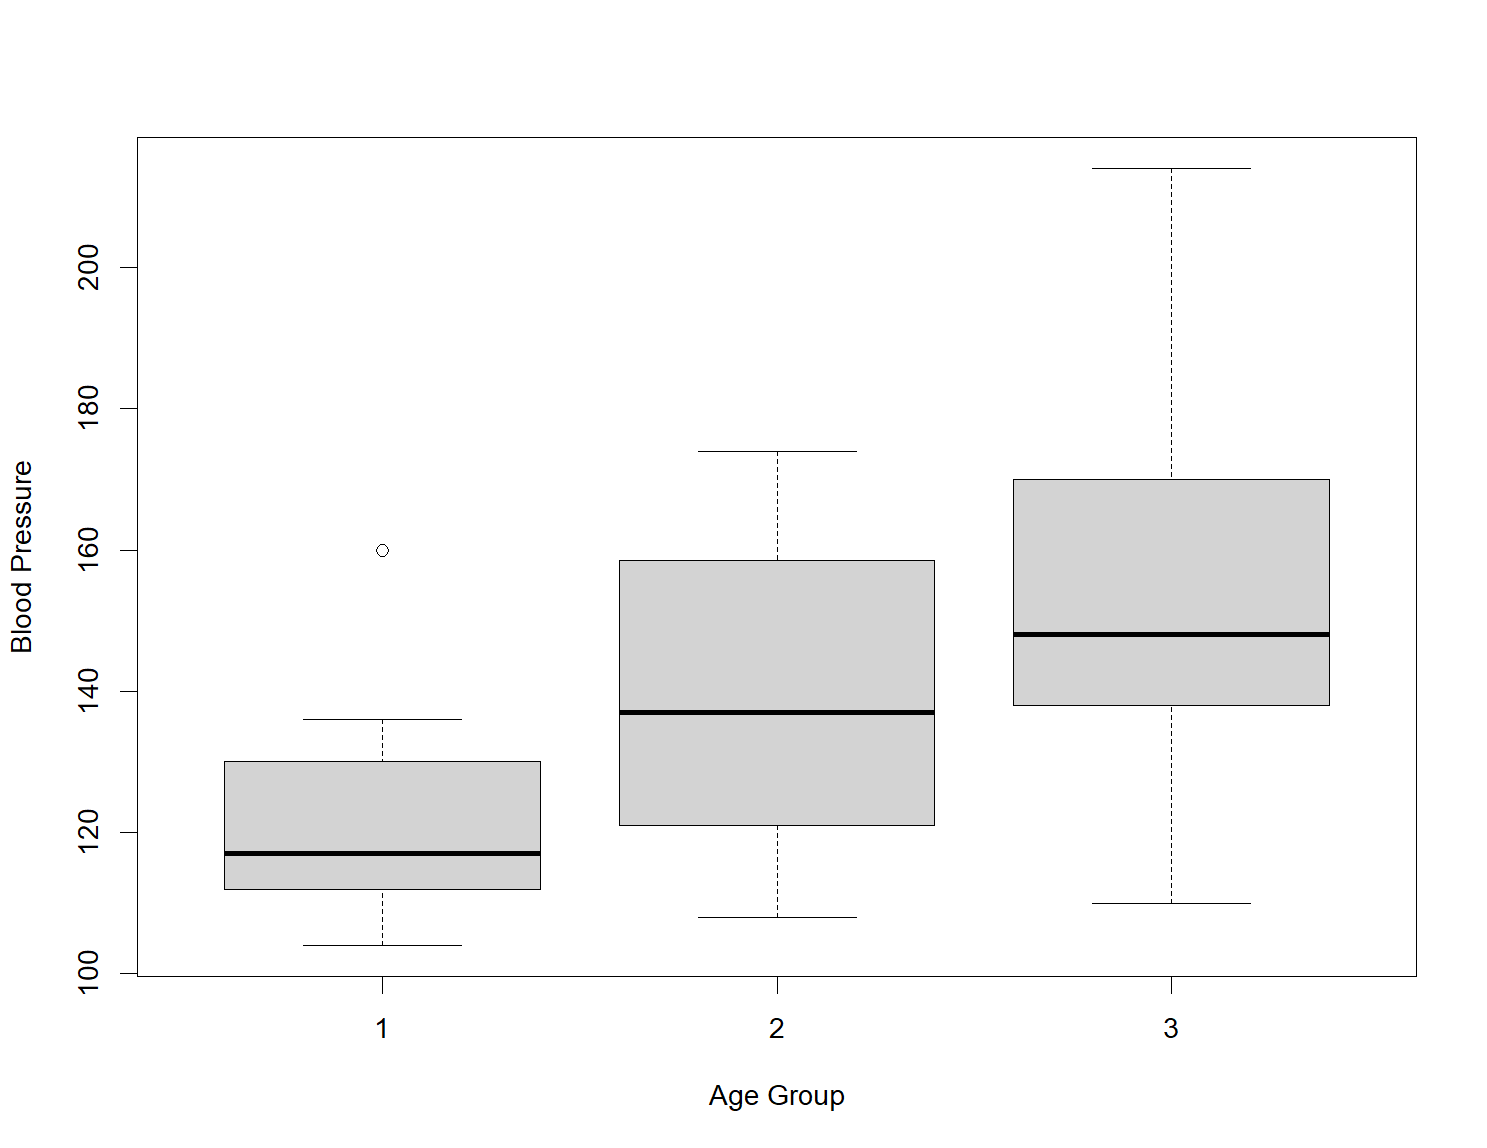
\includegraphics[width=5in, height=4in]{boxplot(2A).png}}
\caption{Box plots of the different age groups.}
\label{fig}
\end{figure}

\subsection*{B. }
We are asked to do a one-way ANOVA to answer the question from A. When using ANOVA we are under the assumption that all observations are independent and that the data from each age group are chosen at random from a normal distributed population. The purpose of the one-way ANOVA is to check if blood pressure varies between the age groups. \


We will test the following hypothesis:
 \begin{equation} 
\begin{split}
&H_0:\mu_1=\mu_2=\mu_3\\
&H_a:\mu_1 \neq \mu_2 \neq \mu_3\\
\end{split}
\end{equation}

 
\begin{table}[H]
\caption{Numerical values of one-way ANOVA test for the 3 age groups.} 
\centering 
\begin{tabular}{c c c c c c } 
\hline\hline 
  & Df & Sum Sq &Mean Sq & F value &Pr(>F)       \\ [0.5ex] 
\hline 
Age group     &2      &6535     &3268 &6.469&0.00426 \\
Residuals        &33   &16670   &505   &        & \\ [1ex] 
\hline\hline
\end{tabular}
\end{table}

 From table 6 we can see that F value is 6.469 and p=0.00426. Large F value and small p value tells us that there is a correlation between age group and blood pressure, and therefore we reject the null hypothesis.  
\subsection*{C. }
Using age group as the categorical predictor variable, we fit a simple linear model. Using treatment-contrast and the youngest group as reference. The youngest group is age group 1 and that will be used as reference, and aging as the treatment. The results are summarized in the table below. 

\begin{table}[H]
\caption{Summary of the linear model with age group as the categorical predictor variable.} 
\centering 
\begin{tabular}{c c c c c } 
\hline\hline 
 & Estimate & Std. Error & t value &  Pr(>|t|)          \\ [0.5ex] 
\hline 
(Intercept)   &122.167   &6.488   &18.829 &2e-16 \\
Age group 2 &16.917   &9.176  &1.844  &< 0.07423 \\
Age group 3 &33   &9.176  &3.596  &0.00104 \\ [1ex] 

\hline 
\multicolumn{5}{c }{Residual standard error: 22.48 on 33 degrees of freedom }\\
\multicolumn{5}{c }{Multiple R-squared:  0.2816,	Adjusted R-squared:  0.2381 }\\
\multicolumn{5}{c }{F-statistic: 6.469 on 2 and 33 DF,  p-value: 0.004263 }\\
\hline\hline
\end{tabular}
\end{table}
 
Reading off p values from table 7, we can see that $p<0.05$ for age group 2 and $p=0.001$ for age group 3. For age group 2, the p value is not significant but the same does not hold for age group 3. Looking at the low $R^2$ for the fit model there might be other factors beside age that also affect blood pressure. One other possibility is that blood pressure and age might have a stronger nonlinear relationship than a linear relationship. But when it comes to only linearity, the same conclusion as in B. holds here to, that there is a significant difference in the mean between the age groups and that age has an effect on blood pressure. 






\pagebreak
\subsection*{Appendix}
\subsection*{R Code}

\begin{lstlisting}[language=R]
#Problem 1.
rm(list = ls())
# Reading the data.
no2.data <- read.table("https://www.uio.no/
studier/emner/matnat/math/STK4900/data/
no2.txt",sep="\t",header=TRUE)

# Assigning parameters to each data type.
log.cars = no2.data$log.cars
log.no2 = no2.data$log.no2
temp = no2.data$temp
wind.speed = no2.data$wind.speed
hour.of.day = no2.data$hour.of.day

#A.
# Printing the data.
no2.data

#Summaries.
summary(log.no2)
summary(log.cars)


#Boxplot for each variable.
boxplot(log.no2, ylab="log.no2")
boxplot(log.cars, ylab="log.cars")

#Scatterplot.
plot(log.cars, log.no2,lwd = 2)      

#B.

#Simple linear fit.
fit = lm(log.no2~log.cars)
summary(fit)

#Plotting all the Data points together with the fitted model.
plot(log.no2~log.cars,lwd = 2)
abline(fit,col = "red",lwd = 3)


#C.
# Partial residual plot, checking for linearity.
par(mfrow = c(1,1))
library(car)
crPlots(fit, terms=~log.cars)

# Residuals vs fitted and sq-rt(standard residuals) vs fitted values.
par(mfrow = c(1,2))
plot(fit,1)
plot(fit,3)

# Histogram of the fitted residuals and box plot of fitted residuals.
par(mfrow = c(1,2))
hist(fit$res,breaks=20)
boxplot(fit$res)

#Normal q-q plot.
par(mfrow = c(1,1))
qqnorm(fit$res); qqline(fit$res)


#D.
# Fitting multiple linear regression models.
# Finding the best model through trial and error.
multi.fit = lm(log.no2~log.cars+temp+wind.speed + log(hour.of.day))
summary(multi.fit)

multi.fit = lm(log.no2~log.cars+temp+wind.speed + hour.of.day)
summary(multi.fit)

multi.fit = lm(log.no2~log.cars+temp+log(wind.speed) + log(hour.of.day))
summary(multi.fit)

#Best model.
multi.fit = lm(log.no2~log.cars+temp+log(wind.speed) + hour.of.day)
summary(multi.fit)

#E.
#Cpr plot.
crPlots(multi.fit, terms=~log.cars+temp+log(wind.speed) + hour.of.day)
\end{lstlisting}

\begin{lstlisting}[language=R]
#Problem 2.
rm(list = ls())
# Reading the data.
blood.data <- read.table("https://www.uio.no
/studier/emner/matnat/math/STK4900/data/blood.txt",
sep=" ",header=TRUE)

#A.
#summary of the different age groups.
summary(subset(blood.data,age==1))
summary(subset(blood.data,age==2))
summary(subset(blood.data,age==3))

#Boxplot of the different age groups.
boxplot(blood.data$Bloodpr  ~ blood.data$age, 
xlab = "Age Group", ylab = "Blood Pressure")

#B.
#One-way ANOVA.
blood.data$age=factor(blood.data$age)
blood.anova = aov(Bloodpr~age,data = blood.data)
summary(blood.anova)

#C.
#Linear fit.
blood.fit = lm(Bloodpr~age,data = blood.data)
summary(blood.fit)
\end{lstlisting}


\end{document}